\documentclass[11pt, english, fleqn, DIV=15, headinclude, BCOR=1cm]{scrartcl}

\usepackage[bibatend]{../header}

\usepackage{lastpage}
\usepackage{multicol}
\usepackage{simplewick}
\usepackage{slashed}
\usepackage{subcaption}

\newcommand\timeorder{\mathscr T}
\newcommand\normorder{\mathscr N}
\newcommand\eye{\mat 1_4}
\newcommand\myslash[1]{\underline{\slashed{\vec{#1}}}}

\hypersetup{
    pdftitle=
}

\graphicspath{{build/}}

\newcounter{totalpoints}
\newcommand\punkte[1]{#1\addtocounter{totalpoints}{#1}}

\newcounter{problemset}
\setcounter{problemset}{2}

\subject{physics617 -- Theoretical Condensed Matter Physics}
\ihead{physics617 -- Problem Set \arabic{problemset}}

\title{Problem Set \arabic{problemset}}

\newcommand\thegroup{Tutor: Ramsés Sánchez}

\publishers{\thegroup}
\ofoot{\thegroup}

\author{
    Martin Ueding \\ \small{\href{mailto:mu@martin-ueding.de}{mu@martin-ueding.de}}
}
\ifoot{Martin Ueding}

\ohead{\rightmark}

\begin{document}

\maketitle

\vspace{3ex}

\begin{center}
    \begin{tabular}{rrr}
        \toprule
        Problem & Achieved points & Possible points \\
        \midrule
        \nameref{homework:1} & & \\
        \nameref{homework:2} & & \\
        \midrule
        %Total & & \arabic{totalpoints} \\
        Total & & 25 \\
        \bottomrule
    \end{tabular}
\end{center}

\vspace{3ex}

\begin{center}
    \begin{small}
        This document consists of \pageref{LastPage} pages.
    \end{small}
\end{center}

\section{Linear chain with next-nearest neighbor hopping}
\label{homework:1}

\subsection{Dispersion}

We are given a linear chain with distance~$a$ between the sites. The there
first- and second-neighbor hopping amplitudes $t_1$ and $t_2$. We will assume
that the hopping amplitudes are real. The situation is depicted in
Figure~\ref{fig:hopping}.

\begin{figure}
    \centering
    \includegraphics{hopping}
    \caption{%
        Hopping amplitudes between the lattice sites.
    }
    \label{fig:hopping}
\end{figure}

Instead of building up a Hamiltonian from (unknown) potential and kinetic
energy we will just use the hopping amplitudes as was done in the in-class
exercise “Tight-binding model on a honeycomb lattice”. The Hamiltonian then
looks like this:
\[
    H =
    - t_1 \sum_{i, j \; \text{nearest neighbors}}
    [c_i^\dagger c_j + \hc]
    - t_2 \sum_{i, j \; \text{next nearest neighbors}}
    [c_i^\dagger c_j + \hc] \,.
\]
There is probably nice notation like $\braket{i, j}$ for the first part. I do
not know how to deal with the second part, so we will just use indices for
that. Then the Hamiltonian will take take the following form:
\[
    H =
    - \sum_i
    [c_i^\dagger c_{j+1} + c_i^\dagger c_{j+2} + \hc] \,.
\]
In total there are four terms which correspond to the four possible hopping
distances of \numlist{+1;+2;-1;-2}. This Hamiltonian has a similar form
compared to the one shown on Monday in class. It is not diagonal and needs to
be diagonalized to give sensible energy eigenvalues. The diagonalization starts
with a Fourier transformation of the ladder operators. It is given as
\[
    c_j = \frac{1}{\sqrt{N}} \sum_k c_k \exp(\iup kaj) \,,
\]
where $N$ is the number of lattice sites, $j$ the lattice site, $k$ is a
momentum and $a$ the spacing of the lattice. Although the imaginary unit~$\iup$
and the index~$i$ can distinguished in print, we try not to mix them too much.
We insert the Fourier expansion into the Hamiltonian and obtain
\begin{align*}
    H
    &= - \frac 1N \sum_{j,k_1,k_2}
    \sbr{
        t_1 c_{k_1}^\dagger \exp(- \iup k_1 a j)
        c_{k_2} \exp(\iup k_2 a [j+1])
        + t_2 c_{k_1}^\dagger \exp(- \iup k_1 a j)
        c_{k_2} \exp(\iup k_2 a [j+2])
    }
    \\&\quad
    + \hc \,.
    \intertext{%
        The exponentials can be joined to yield
    }
    &= - \frac 1N \sum_{j,k_1,k_2}
    \sbr{
        t_1 c_{k_1}^\dagger c_{k_2} \exp(\iup a [- k_1 j + k_2 [j+1]])
        + t_2 c_{k_1}^\dagger c_{k_2} \exp(\iup a [- k_1 j + k_2 [j+2]])
    } + \hc \,.
    \intertext{%
        The parts with $j$ can be factored out.
    }
    &= - \frac 1N \sum_{j,k_1,k_2}
    \sbr{
        [t_1 + t_2] c_{k_1}^\dagger c_{k_2} \exp(\iup a [k_2 - k_1] j)
        + t_1 c_{k_1}^\dagger c_{k_2} \exp(\iup a k_2)
        + t_2 c_{k_1}^\dagger c_{k_2} \exp(2 \iup a k_2)
    }
    \\&\quad
    + \hc
    \intertext{%
        The first exponential together with $\sum_j/N$ will give a
        $\delta_{k_1k_2}$. The other terms will just obtain a factor $N$ which
        cancels the one up front. The sum over $k_1$ can be directly removed
        with the Kronecker symbol, then. The only things left then are
    }
    &= - \sum_{k_2}
    \sbr{
        [t_1 + t_2] c_{k_2}^\dagger c_{k_2}
        + t_1 c_{k_1}^\dagger c_{k_2} \exp(\iup a k_2)
        + t_2 c_{k_1}^\dagger c_{k_2} \exp(2 \iup a k_2)
    } + \hc \,.
    \intertext{%
        The first term apparently is the energy for a single wave. The two
        others are terms which bind two different momenta together. We can
        write this as a matrix where we have to consider the hermitian
        conjugate terms such that we obtain a hermitian matrix. All the terms
        (with $k_1 = k_2$) will be on the diagonal. On the diagonal, the
        hermitian conjugate will convert the exponentials into cosine
        functions. The off-diagonal terms will only contain the last two terms.
        The Hamiltonian then assumes the form
    }
    &= - \sum_{k_2}
    \begin{pmatrix}
        c_{k_1} \\ c_{k_2}
    \end{pmatrix}^\dagger
    \mat M
    \begin{pmatrix}
        c_{k_1} \\ c_{k_2}
    \end{pmatrix} \,,
\end{align*}
where
\[
    \mat M = 
    \begin{pmatrix}
        [t_1 + t_2][1 + 2 \cos(ak_2) + 2 \cos(2 ak_2)] &
        t_1 \exp(\iup a k_2) + t_2 \exp(2 \iup a k_2)
        \\
        t_1 \exp(- \iup a k_2) + t_2 \exp(- 2 \iup a k_2)
        & [t_1 + t_2][1 + 2 \cos(ak_2) + 2 \cos(2 ak_2)]
    \end{pmatrix} \,.
\]
We now want to diagonalize this matrix in order to get the energy eigenvalues.
This amounts to computing the characteristic polynomial.
\[
    \cbr{[t_1 + t_2][1 + 2 \cos(ak_2) + 2 \cos(2 ak_2)] - \lambda}^2
    - \abs{t_1 \exp(\iup a k_2) + t_2 \exp(2 \iup a k_2)}^2
    \overset != 0
\]
One can pull the modulus squared to the other side and take the square root.
The term with the many square brackets needs to be put to the other side as
well. The two solutions of the equation are
\[
    \lambda_\pm
    = 2 [t_1 + t_2][1 + 2 \cos(ak_2) + 2 \cos(2 ak_2)]
    \pm \sqrt{t_1^2 + t_2^2 + 2 t_1 t_2 \cos(ak_2)} \,.
\]
The energy depending on the momentum~$E(k_2)$ then is the negative of this.
This band structure is shown in Figure~\ref{fig:linear-band} for two values of
$t_1$ and $t_2$.

\begin{figure}
    \begin{subfigure}[c]{0.5\linewidth}
        \centering
        \includegraphics{linear-band}
        \caption{%
            $t_1 = 1$, $t_2 = 1$
        }
        \label{fig:linear-band/1}
    \end{subfigure}
    \begin{subfigure}[c]{0.5\linewidth}
        \centering
        \includegraphics{band-3}
        \caption{%
            $t_1 = \num{0.5}$, $t_2 = \num{-0.64}$
        }
        \label{fig:linear-band/2}
    \end{subfigure}
    \caption{%
        Band structure of the linear chain within the first Brillouin zone. The
        bold line is the solution where the square root is subtracted (instead
        of added).
    }
    \label{fig:linear-band}
\end{figure}

\subsection{Number of minima}

The number of minima depends on the two parameters $t_1$ and $t_2$. If both are
taken positive, the bands always looks similar to
Figure~\ref{fig:linear-band/1}. Then the number of minima always is four. When
one parameter becomes negative, the number of minima changes. Depending on the
way minima at the boundary count there are between three and five minima as can
be seen in Figure~\ref{fig:linear-band/2}. In the special case discussed in the
next part of this problem, there are only two minima in the lower band. See
Figure~\ref{fig:band-3} for a graph of that case.

One can solve for the derivative of the energy and set it to zero. Except for
$k_2 = 0$ all the points of vanishing slope are complicated expressions. I
assume that this is not really what was asked here \emph{or} my energy bands
are wrong.

\subsection{Density of states}

I must admit that I first thought that “DOS” is supposed to stand for:

\begin{itemize}
    \item Denial of Service
    \item Degrees of Separation
    \item Disk Operating System
\end{itemize}

Only then later I realized that it is “Density of States” here :-).

\begin{figure}
    \centering
    \includegraphics{linear-band-0_5__-0_5}
    \caption{%
        Band structure with the special values $t_1 = \num{0.5}$, $t_2 =
        \num{-0.5}$.
    }
    \label{fig:band-3}
\end{figure}

The special values for $t_1$ and $t_2$ simplify the band structure drastically.
The two bands are shown in Figure~\ref{fig:band-3}. It now is
\[
    E(k_2) = \mp \sqrt{\frac 12 + \frac 12 \cos(a k_2)} \,.
\]
The inverse of this is
\[
    k_2 = \frac 1a \arccos(2 E^2 - 1) \,.
\]
Taking the derivative of the energy we have
\[
    E'(k_2) = \pm \frac{a \sin(a k_2)}{4 \sqrt{\frac 12 + \frac 12 \cos(a
    k_2)}} \,.
\]
Then the density of states is
\[
    D(E) = \frac{1}{2 \piup} \frac{1}{E'(k_2)}
\]
which has to be evaluated at the point where $k_2(E)$, i.e.\ the inverse
function in the reciprocal derivative. The expression for $\sin(\arccos(x))$
can be derived using the suggestive labeling of the triangle's vertices shown
in Figure~\ref{fig:triangle} as well as the Pythagorean theorem.

\begin{figure}
    \centering
    \includegraphics{triangle}
    \caption{%
        Derivation of $\sin(\arccos(x)) = \sqrt{1 - x^2}$.
    }
    \label{fig:triangle}
\end{figure}

Putting all together we have a density of states
\[
    D(E) = \mp \frac{\sqrt{\frac 12 + \frac 12 [2 E^2 - 1]}}{\piup a E \sqrt{1 -
    E^2}} \,.
\]
One of the two branches is shown in Figure~\ref{fig:dos/2}. It has a jump at $E
= 0$ which makes sense when compared to Figure~\label{fig:band-3}. The density
of states is some sort of histogram of the band structure to the ordinate axis.
At $E = 0$ the two bands just barely meet such that there is no point there,
really. Perhaps one should carefully look at the limit $E \to 0$ as the
function might not have a jump after all. Then going to slightly higher
energies~$E$ there are a couple of states in the four intersections of the band
with the horizontal line where $E$ is a small constant value. Then at $E \to
\pm 1$ the density of states diverges as the bands become horizontal. A
horizontal band with a continuous density of states per arc length or momentum
(almost the same at vanishing slope) will have lots of states with the exact
same energy. Therefore the density diverges there.

\begin{figure}
    \begin{subfigure}[t]{0.47\linewidth}
        \centering
        \includegraphics{dos2}
        \caption{%
            Density function with sign. One can see that it has a jump at $E =
            0$.
        }
        \label{fig:dos/2}
    \end{subfigure}
    \hfill
    \begin{subfigure}[t]{0.47\linewidth}
        \centering
        \includegraphics{dos}
        \caption{%
            Absolute value of the previous function such that is is always
            positive. At $E = 0$ the function takes the value 0.
        }
        \label{fig:dos/1}
    \end{subfigure}
    \caption{%
        Density of states in the linear chain.
    }
    \label{fig:dos}
\end{figure}

\section{Tight-binding model on a kagomé lattice}
\label{homework:2}

\subsection{Dispersion relation}

\begin{figure}
    \begin{subfigure}[c]{0.48\linewidth}
    \centering
    \includegraphics{kagome-unit}
    \caption{%
        Unit cell of the kagomé lattice. Only black sites are included in the
        unit cell. The sites are labeled, it can be seen that there are three
        sites in the unit cell.
    }
    \label{fig:kagome-unit}
    \end{subfigure}
    \hfill
    \begin{subfigure}[c]{0.48\linewidth}
    \centering
    \includegraphics{neighbors}
    \caption{%
        Neighbor directions from site~1 in the unit cell. The jump $2
        \leftrightarrow 3$ can be constructed by a sum of these vectors.
    }
    \label{fig:neighbors}
    \end{subfigure}
    \caption{%
        Kagomé lattice with unit cell and next neighbors.
    }
\end{figure}

This lattice was also covered on the first sheet, so we will copy some of the
results derived there as well as the figures. We chose the unit cell as shown
in Figure~\ref{fig:kagome-unit}. The Bravais vectors are
\[
    \vec a_1 = a
    \begin{pmatrix}
        1 \\ 0
    \end{pmatrix}
    \eqnsep
    \vec a_2 = a
    \begin{pmatrix}
        1/2 \\ \sqrt{3} / 2
    \end{pmatrix} \,.
\]
The two next-neighbor translation vectors are
\[
    \vec \delta_1 = \frac a2
    \begin{pmatrix}
        1 \\ 0
    \end{pmatrix}
    \eqnsep
    \vec \delta_2 = \frac a2
    \begin{pmatrix}
        1/2 \\ \sqrt{3} / 2
    \end{pmatrix} \,.
\]
Those vectors are illustrated in Figure~\ref{fig:neighbors}. If the unit cell
has been chosen differently, those vectors might be rotated by a multiple of
$\piup/3$. This should not change the derivation of the band structure much.
Later in the explicit path within the first Brillouin zone that might become a
problem.

We construct the Hamiltonian using next neighbors:
\begin{align*}
    H
    &= -t \sum_{\bracket{x, l, y, l'}} c_{xl}^\dagger c_{yl'} + \hc \,.
    \intertext{%
        Now we insert the Fourier transform of the ladder operators.
    }
    &= -\frac{t}{N_\mathrm c} \sum_{\bracket{x, l, y, l'}, k, k'} c_{kl}^\dagger c_{k'l'}
    \exp(-\iup k \cdot [\vec x + \vec l]) \exp(\iup k' \cdot [\vec y + \vec l']) + \hc
    \intertext{%
        There are too many summation indices for this to be useful. We will set
        $\vec x = \vec y$ and then only go to the next neighbors using the
        $\vec l$ and $\vec l'$.
    }
    &= -\frac{t}{N_\mathrm c} \sum_{\bracket{x, l, l'}, k, k'} c_{kl}^\dagger c_{k'l'}
    \exp(-\iup [\vec k - \vec k'] \cdot \vec x )
    \exp(-\iup \vec k \cdot \vec l)
    \exp(\iup \vec k' \cdot \vec l') + \hc
    \intertext{%
        This will give us a Kronecker-symbol from the exponentials. Using it
        directly to get rid of the $\vec k'$ sum we obtain
    }
    &= - t \sum_{\bracket{l, l'}, k} c_{kl}^\dagger c_{kl'}
    \exp(-\iup \vec k \cdot [\vec l - \vec l']) + \hc \,.
    \intertext{%
        The sum over all next neighbors amounts to including all the
        transitions between the neighbors shown in Table~\ref{tab:transitions}.
        For some reason the case $\vec l = \vec l'$ is not included in the
        solution on Monday. We do not include that here and have a traceless
        matrix. What is the underlying reason for that? We have $\vec \delta_l
        = \vec l - \vec l'$ and then introduce the shorthand $k_i = \vec k
        \cdot \vec \delta_l$. We obtain two terms for the direction forward and
        backwards. Both terms together give a cosine.
    }
    &= - 2 t \sum_{k}
    \sbr{
        c_{k2}^\dagger c_{k1} \cos(k_1)
        + c_{k3}^\dagger c_{k1} \cos(k_2)
        + c_{k3}^\dagger c_{k2} \cos(k_1 - k_2)
    }
    + \hc
    \intertext{%
        This looks sufficiently parallel to the derivation of the honeycomb
        lattice presented in class. We put that into a hermitian matrix.
    }
    &= -2 t \sum_{k}
    \begin{pmatrix}
        c_{k1} \\ c_{k2} \\ c_{k2}
    \end{pmatrix}^\dagger
    \begin{pmatrix}
        0 & \cos(k_1) & \cos(k_2) \\
        \cos(k_1) & 0 & \cos(k_1 - k_2) \\
        \cos(k_2) & \cos(k_1 - k_2) & 0
    \end{pmatrix}
    \begin{pmatrix}
        c_{k1} \\ c_{k2} \\ c_{k2}
    \end{pmatrix}
\end{align*}

\begin{table}
    \centering
    \begin{tabular}{ccc}
        \toprule
        From & To & Vector \\
        \midrule
        1 & 2 & $\delta_1$ \\
        1 & 2 & $-\delta_1$ \\
        1 & 3 & $\delta_2$ \\
        1 & 3 & $-\delta_2$ \\
        2 & 3 & $\delta_2 - \delta_1$ \\
        2 & 3 & $\delta_1 - \delta_2$ \\
        \bottomrule
    \end{tabular}
    \caption{%
        Allowed transitions between the next neighbors.
    }
    \label{tab:transitions}
\end{table}

The eigenvalues of this matrix have to be found. \emph{Mathematica} happily did
that for us. They are
\[
    \lambda = 0
    \eqnsep
    \lambda_\pm = \frac 12 \pm \frac 12 \sqrt{3 + 2 \cos(2 k_1) + 2 \cos(2 k_1
    - 2 k_2) + 2 \cos(2 k_2)} \,.
\]
The shorthands $k_1$ and $k_2$ have to be expanded. We have
\[
    k_1 = \frac a2 k^1
    \eqnsep
    k_2 = \frac a4 [k^1 + \sqrt 3 k^2] \,,
\]
where the $k^i$ are the components of $\vec k$ whereas the $k_i$ are the
shorthands. This can be inserted into the expression for $\lambda_\pm$ and then
we yield $\lambda_\pm(\vec k)$ which we can plot in the reciprocal lattice.


%The reciprocal lattice is
%\[
%    \vec b_1 = \frac{2\piup}{a}
%    \begin{pmatrix}
%        1 \\ -1 / \sqrt{3}
%    \end{pmatrix}
%    \eqnsep
%    \vec b_2 = \frac{2\piup}{a}
%    \begin{pmatrix}
%        0 \\ 2 / \sqrt{3}
%    \end{pmatrix} \,.
%\]

Figure~\ref{fig:band-3d} shows a 3D-plot of the two eigenvalues which are the
bands (except for constants factors).

\begin{figure}
    \begin{subfigure}[c]{0.48\linewidth}
    \centering
    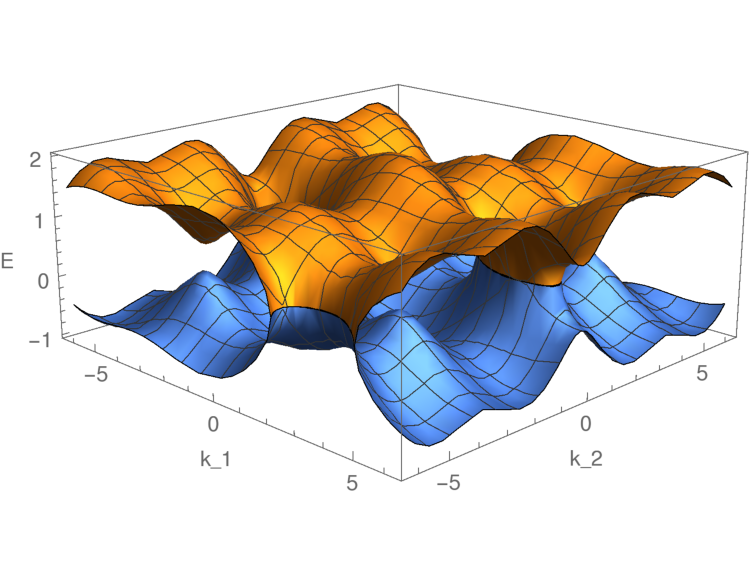
\includegraphics[width=\linewidth]{2-Eigenvalues.pdf}
    \caption{%
        \emph{Mathematica} version
    }
    \label{fig:}
    \end{subfigure}
    \hfill
    \begin{subfigure}[c]{0.48\linewidth}
    \centering
    \includegraphics{3d}
    \caption{%
        \emph{pgfplots} version. Unbounded points had to be skipped which makes
        the package also drop the surface segment with the options tried.
    }
    \label{fig:}
    \end{subfigure}
    \caption{%
        Upper and lower band as functions of the two-vector $\vec k$. One can
        see that interesting surfaces which form as well as a couple points
        where both bands nearly touch.
    }
    \label{fig:band-3d}
\end{figure}

\subsection{Band structure}

The band structure is shown in Figure~\ref{fig:band-3d} in a 3D representation
which is not very helpful to get an exact feeling for certain types of wave
vectors. Therefore it is common to look at the bands along a certain path in
the reciprocal space. The path we will look at is shown in
Figure~\ref{fig:along-path/1}. Depending on the choice of unit cell above the
reciprocal space can differ. In the worst case the coordinates do not make for
an interesting band. The resulting section through the band-surfaces is shown
in Figure~\ref{fig:along-path/2}.

\begin{figure}
    \begin{subfigure}[c]{0.48\linewidth}
    \centering
    \includegraphics{path}
    \caption{%
        Chosen path in reciprocal space.
    }
    \label{fig:along-path/1}
    \end{subfigure}
    \hfill
    \begin{subfigure}[c]{0.48\linewidth}
    \centering
    \includegraphics{along-path}
    \caption{%
        Bands along the path.
    }
    \label{fig:along-path/2}
    \end{subfigure}
    \caption{%
        Band structure along path.
    }
    \label{fig:along-path}
\end{figure}

\end{document}

% vim: spell spelllang=en tw=79
